\section{Descripción general del sistema}

El diseño implementado corresponde a un sistema UART extendido con capacidades de procesamiento mediante una \textbf{Unidad Aritmético-Lógica (ALU)}. El bloque superior \texttt{top} integra todos los módulos que lo componen y define el flujo de datos completo desde la entrada serie (\texttt{rx}) hasta la salida (\texttt{tx}).

\subsection{Bloque \texttt{top}}
El módulo \texttt{top} actúa como entidad principal, interconectando:
\begin{itemize}
    \item El generador de baudios, encargado de derivar la señal de muestreo \texttt{sample\_tick}.
    \item El receptor UART (\texttt{uart\_rx}), que reconstruye bytes a partir de la señal serie entrante.
    \item Dos memorias FIFO: una para los datos recibidos (FIFO RX) y otra para los datos a transmitir (FIFO TX).
    \item El decodificador de instrucciones (\texttt{rv\_decoder}), que clasifica la instrucción (tipo R/I), extrae campos (\texttt{rd}, \texttt{rs1}, \texttt{rs2}, \texttt{imm}) y selecciona \texttt{alu\_op}.
    \item El banco de registros (\texttt{regfile}), que provee operandos por dirección y recibe el resultado en \texttt{rd} bajo señal de escritura, preservando el registro nulo.
    \item El módulo de interfaz (\texttt{rv\_interface}), que ensambla una instrucción de 32 bits con 4 bytes UART, coordina las lecturas/escrituras del \texttt{regfile}, alimenta la ALU, realiza el \textit{write-back} y, si corresponde, genera la respuesta hacia la FIFO TX.
    \item La ALU, que realiza las operaciones aritméticas y lógicas definidas.
    \item El transmisor UART (\texttt{uart\_tx}), que serializa los datos de salida.
\end{itemize}

\newpage

\subsection{Esquemático general}
La Figura~\ref{fig:uart-general} muestra un diagrama de bloques típico de un sistema UART completo, donde se observa la integración del generador de baudios, los bloques de transmisión y recepción, y las memorias FIFO.

\begin{figure}[H]
    \centering
    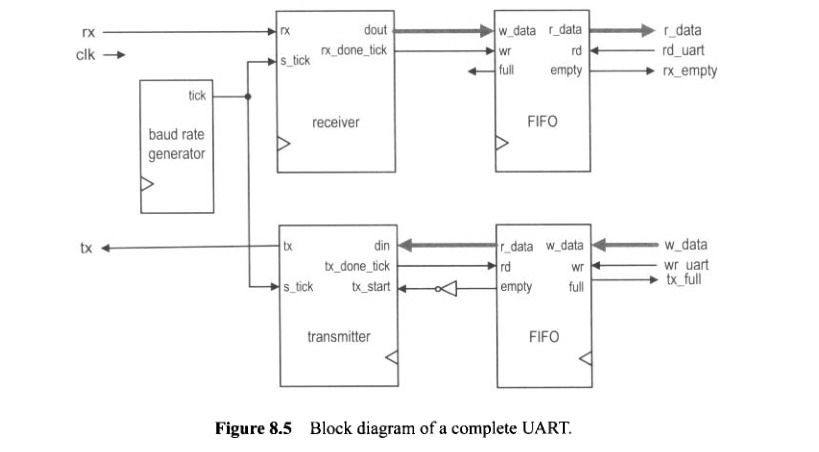
\includegraphics[width=0.75\textwidth]{img/completeUART.jpeg}
    \caption{Diagrama de bloques de un UART completo \cite{libroUART}.}
    \label{fig:uart-general}
\end{figure}

\subsection{Flujo de datos}
El flujo de información en el sistema sigue la siguiente secuencia:
\begin{enumerate}
    \item Los datos ingresan por la línea \texttt{rx} y son muestreados por el \texttt{uart\_rx}.
    \item Los bytes reconstruidos se almacenan en la \textbf{FIFO RX}.
    \item La \textbf{interfaz} ensambla una \textbf{instrucción de 32 bits} a partir de cuatro bytes UART y la entrega al \textbf{decodificador}.
    \item El \textbf{decodificador} determina el tipo (R/I), extrae \texttt{rd}, \texttt{rs1}, \texttt{rs2} e \texttt{imm}, y selecciona \texttt{alu\_op}.
    \item La \textbf{interfaz} coordina el acceso al \textbf{regfile} para leer operandos (\texttt{rs1} y, según el caso, \texttt{rs2} o \texttt{imm}) y \textbf{alimenta la ALU}.
    \item La \textbf{ALU} procesa los operandos y genera un \textbf{resultado}.
    \item Si corresponde (tipo R/I y \texttt{rd}\(\neq 0\)), la \textbf{interfaz} realiza el \textbf{write-back} en el \texttt{regfile} (escritura en \texttt{rd}).
    \item La \textbf{interfaz} puede formar una \textbf{respuesta} y escribirla en la \textbf{FIFO TX}.
    \item Finalmente, el \texttt{uart\_tx} serializa el dato y lo envía por la línea \texttt{tx}.
\end{enumerate}
